\documentclass[11pt,
  paper=a4, 
  bibliography=totocnumbered,
	captions=tableheading,
	BCOR=10mm
]{scrreprt}

\usepackage[utf8]{inputenc}

 
 
\usepackage[onehalfspacing]{setspace}
\usepackage{csquotes} % Context sensitive quotation.
\usepackage{amsmath} % Standard math.
\usepackage{amsthm} % Math theorems.
\usepackage{amssymb} % More math symbols.
\theoremstyle{definition}
\newtheorem{definition}{Definition}[chapter]
 
\usepackage[section]{placeins} % Keep floats in the section they were defined in.
\usepackage{tabularx}
\usepackage{booktabs} % Scientific table styling.
\usepackage{floatrow} % Option for keeping floats in the place they were defined in the code.
\floatsetup[table]{style=plaintop}
\usepackage{hyperref} % Hyperlinks.
\usepackage[all]{nowidow} % Prevent widows and orphans.
\usepackage{xstring} % logic string operations
\usepackage{bbm} % \mathbb on numerals.
\usepackage{csquotes}
\usepackage{mathtools}
\usepackage[ruled,vlined]{algorithm2e} % Pseudocode
\usepackage{scrhack} % Make warning go away.

\usepackage{graphicx}
\usepackage{subcaption} % Subfigures with subcaptions.
\usepackage{authoraftertitle} % Make author, etc., available after \maketitle
\usepackage{listofitems}
\usepackage{blindtext} % Placeholder text.
\usepackage{comment} % allows block comments
\usepackage[automake, nopostdot, nonumberlist,acronym, toc]{glossaries} % glossary for definitions and acronyms, without dot after entry and page reference 

\makeglossaries % Generate the glossary

% \PassOptionsToPackage{obeyspaces}{url}%
\usepackage[backend=bibtex,% 
style=nature,% 
doi=true,isbn=false,url=false, eprint=false]{biblatex}
% \renewbibmacro*{url}{\printfield{urlraw}}

\addbibresource{bib/library.bib}

\DeclareStyleSourcemap{
  \maps[datatype=bibtex, overwrite=true]{
    \map{
      \step[fieldsource=url, final]
      \step[typesource=misc, typetarget=online]
    }
    \map{
      \step[typesource=misc, typetarget=patent, final]
      \step[fieldsource=institution, final]
      \step[fieldset=holder, origfieldval]
    }
  }
}

%\linespread{1.5} % set line spacing
 
\usepackage{listings} % rendering program code
\lstset{% general command to set parameter(s)
	basicstyle=\ttfamily\color{grey},          % print whole listing small
	keywordstyle=\color{black}\bfseries\underbar,
	% underlined bold black keywords
	identifierstyle=,           % nothing happens
	commentstyle=\color{white}, % white comments
	stringstyle=\ttfamily,      % typewriter type for strings
	showstringspaces=false}     % no special string spaces


\DeclareFontFamily{U}{mathx}{\hyphenchar\font45}
\DeclareFontShape{U}{mathx}{m}{n}{
      <5> <6> <7> <8> <9> <10>
      <10.95> <12> <14.4> <17.28> <20.74> <24.88>
      mathx10
      }{}
\DeclareSymbolFont{mathx}{U}{mathx}{m}{n}
\DeclareFontSubstitution{U}{mathx}{m}{n}
\DeclareMathSymbol{\bigtimes}{1}{mathx}{"91}

 

%%% Custom definitions %%%
% Shorthands
\newcommand{\ie}{i.\,e.~}
\newcommand{\eg}{e.\,g.~}
\newcommand{\ind}{\mathbbm{1}}
% Functions
\newcommand{\tpow}[1]{\cdot 10^{#1}}
\newcommand{\figref}[1]{(Figure \ref{#1})}
\newcommand{\figureref}[1]{Figure \ref{#1}}
\newcommand{\tabref}[1]{(Table \ref{#1})}
\newcommand{\tableref}[1]{Table \ref{#1}}
\newcommand{\secref}[1]{%
	\IfBeginWith{#1}{chap:}{%
		(cf. Chapter \ref{#1})}%
		{(cf. Section \ref{#1})}%
		}
\newcommand{\sectionref}[1]{%
	\IfBeginWith{#1}{chap:}{%
		Chapter \ref{#1}}%
		{\IfBeginWith{#1}{s}{%
			Section \ref{#1}}%
			{[\PackageError{sectionref}{Undefined option to sectionref: #1}{}]}}}
\newcommand{\chapref}[1]{(see chapter \ref{#1})}
\newcommand{\unit}[1]{\,\mathrm{#1}}
\newcommand{\unitfrac}[2]{\,\mathrm{\frac{#1}{#2}}}
\newcommand{\codeil}[1]{\lstinline{#1}}{} % wrapper for preventing syntax highlight error
\newcommand{\techil}[1]{\texttt{#1}}
\newcommand{\Set}[2]{%
  \{\, #1 \mid #2 \, \}%
}
% Line for signature.
\newcommand{\namesigdate}[1][5cm]{%
	\vspace{5cm}
	{\setlength{\parindent}{0cm}
	\begin{minipage}{0.3\textwidth}
		\hrule 
		\vspace{0.5cm}
		{\small city, date}
	\end{minipage}
	 \hfill
	\begin{minipage}{0.3\textwidth}
		\hrule
		\vspace{0.5cm}
	    {\small signature}
	\end{minipage}
	}
}
% Math
\newcommand{\TP}{\text{TP}}
\newcommand{\TN}{\text{TN}}
\newcommand{\FP}{\text{FP}}
\newcommand{\FN}{\text{FN}}

% Automatically use the first sentence in a caption as the short caption.
\newcommand\slcaption[1]{\setsepchar{.}\readlist*\pdots{#1}\caption[{\pdots[1].}]{#1}}

% Variables. 
% Adapt if necessary, use to refer to figures and graphics.
\def \figwidth {0.9\linewidth}
\graphicspath{ {./graphics/figures/}{./graphics/figures/} } % Path to figures and images.


% Customizations of existing commands.
\renewcommand{\vec}[1]{\mathbf{#1}}
% Capitalized \autoref names.
\renewcommand*{\chapterautorefname}{Chapter}
\renewcommand*{\sectionautorefname}{Section}

\usepackage{caption}
\DeclareCaptionType{equ}[Equations][List of Equations]
\usepackage{capt-of}
\usepackage{listings}

\title{On the Potential of Recurrent Structures for Semantic Video Segmentation with Deep Networks}
\author{Sven Groen}



%Numbering of Figures
\usepackage{chngcntr}
\counterwithout{figure}{chapter}
\counterwithout{equ}{chapter}

\begin{document}

\begin{titlepage}
	\begin{flushleft}
		Universität Osnabrück\\
		Fachbereich Humanwissenschaften\\
		Institute of Cognitive Science
	\end{flushleft}

	\vspace{2cm}
	\centering{
		Bachelorthesis\vspace{1cm}\\
		\textbf{\Large{\MyTitle}}
		\vspace{1cm}\\
		\begin{tabular}{c}
			\MyAuthor                          \\
			970219                            \\
			Bachelor's Program Cognitive Science \\
			June 2020 - September 2020
		\end{tabular}}
	\vspace{1cm}

	\begin{tabular}{ll}
		First supervisor:  & Dr. Ulf Krumnack          \\
		                   & Institute of Cognitive Science            \\
		                   & Osnabrück                \\\\
		Second supervisor: & Manuel Kolmet         \\
		                   & IMANOX GmbH  \\
		                   & Berlin 
	\end{tabular}

\end{titlepage}


\chapter*{Declaration of Authorship}
I hereby certify that the work presented here is, to the best of my knowledge and belief, original and the result of my own investigations, except as acknowledged, and has not been submitted, either in part or whole, for a degree at this or any other university.

\namesigdate
\pagenumbering{gobble}
\pagebreak

\begin{abstract}
	\textbf{\LARGE{Abstract}}\\\\
	%TODO summarize the main objectives and outcomes of your work. The abstract should fit on one page.
	This is the abstract.
\end{abstract}




\tableofcontents
\listoffigures
\listoftables
\listofequs


\chapter{Introduction}
\pagenumbering{arabic}
\section{Motivation} \label{sec:Motivation}

Humans are capable of understanding and interpreting their environment based on visual information without any effort in split seconds. (TODO QUELLE?)
In computer science the field of \textit{Computer Vision} aims to enable computers to achieve a human visual system like performance \cite{Huang1997}.
Deep learning approaches have demonstrated in the last couple of years that they are able to outperform previous approaches towards computer vision problems \cite{Voulodimos2018, Garcia-Garcia2018}.
Understanding the semantic context of an image on a pixel level and segmenting it into its semantic parts is a heavily researched topic in the field of computer vision called \textit{Semantic Segmentation} \cite{Minaee2020, Forsyth2003}.

Potential applications range widely, from autonomous driving over medical image analysis \cite{Minaee2020} to video effects for the film industry.
Semantic Segmentation can not only be applied to single images, but also to video data or 3D data \cite{Garcia-Garcia2018}.
Classical videos are a continuous stream of individual images, called frames, that are usually temporally dependent from another.
Meaning, that each frame is likely to be very similar to its predecessors and its successor frame.
Applying segmentation models on individual frames without the temporal context can cause flickering effects between two frames or sudden incorrect segmentation in single frames of the video sequence \cite{Pfeuffer2_2019}.
This work will investigate whether this similarity between neighboring frames can be used to improve the segmentation map produced by a deep learning algorithm.
This problem is tackled by adding \gls{ru} into existing algorithms to enable the use of the temporal context the frame is in.
The realization of this solution is done in a real world use-case scenario based on a problem offered by IMANOX.

\section{Cooperation with IMANOX}\label{sec:Imanox}
This project is realized in cooperation with \href{https://www.Imanox.de/}{IMANOX}. 
IMANOX is a Berlin-based startup that developed a smart photo booth for expositions, events and promotions. 
The photo booth enables customers virtual product placements using augmented and mixed reality. 
Main features are hand-tracking, digital masks and changing virtual backgrounds.


\subsection{Segmentation use case scenario}\label{sec:Usecase}
One feature offered by the photo booth is to replace the background the user is standing in front of by a virtual background the user can choose.
The actual real world background the person is standing in front of varies across customers.
Currently, the photo booth is using a built in Kinect \gls{rgb}-Depth camera that measures the distance of objects by casting infrared illumination onto the scene and indirectly measuring the time it takes to travel back to the camera \cite{Cruz2012}. 
However, the camera struggles with correctly predicting the depth in certain situations. 
The reasons for this are numerous. 
Pixels might get undersaturated (signal is not strong enough) or oversaturated (signal is too strong) leading to pixels being rendered as invalid and no depth information is provided \cite{Microsoft2019}.
Other artifacts occur due to the geometry of the scene with objects being too far away or having a transparent or matte surface \cite{Kim2014}. 
For example, the sensors of the camera might receive signals from multiple locations in the scene, leading to an ambiguous depth \cite{Microsoft2019}. 
Especially around the edges and borders of objects pixels contain mixed signals from fore- and background, leading to blurred outlines \cite{Kim2013}.
In the current version of the photo booth, alpha values (0 to 1) are calculated based on the data from the depth sensor. 
This is done by applying an alpha matting algorithm \cite{Gastal2010} to the raw depth data.
Objects that are considered to be located in the foreground receive high alpha values while the background is considered to have an alpha value of 0, making it transparent. 
In this way, the background can be virtually replaced without affecting the objects in the foreground. 
Due to the described inaccurate data that is given by the depth sensor, the resulting foreground background segmentation is of low quality. 
The edges and borders of the objects or people in the scene are not sharp and often misclassified. 
Moreover, it can be observed that the exact boarder of an object varies in between the different frames leading to a flickering effect around object borders.


\section{Semantic Segmentation}

\textcite{Szeliski2011} refers to image segmentation as "the task of finding groups of pixels that 'go together'" (\cite{Szeliski2011}, p. 237).
How the pixels are \textit{grouped together} can be achieved in different ways.
In the classical image classification tasks, the task is to simply name the objects that can be seen in an image.
Semantic image segmentation extends this problem further, referring to a pixel-wise classification of an image \cite{Minaee2020}.
Each pixel in an image is assigned to one category label given a set of categories.

However, individual instances of an object in one image are not differentiated but labelled as one class.
Instance segmentation combines a pixel-wise classification (similar to semantic segmentation) with an additional object detection and localization, differentiating each individual instance of a class \cite{Minaee2020}.
Given the provided use-case scenario in section \ref{sec:Usecase}, only binary semantic segmentation is necessary.
Detailed information about which objects are in the scene is not required.

\begin{figure}[H]
	\centering
	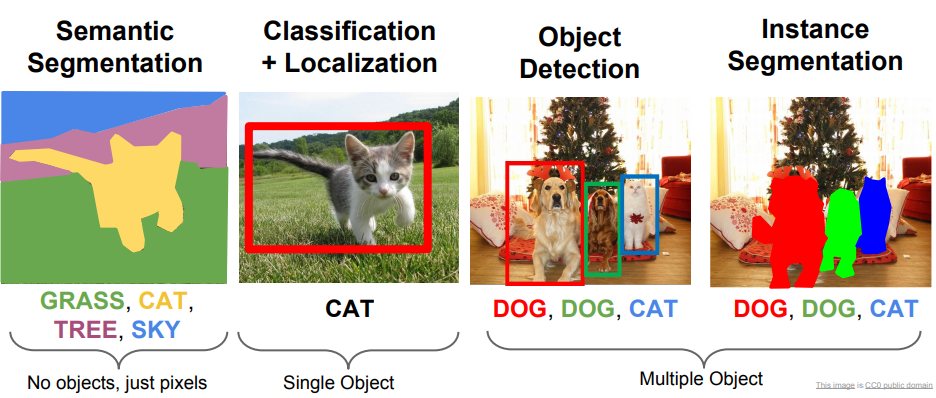
\includegraphics[width=\figwidth]{Computer_Vision_Tasks}
	\caption[Overview of Computer Vision Tasks]{
		Overview of Computer Vision Tasks. (\textcite{Fei-Fei2017}, Slide 17).
		\label{fig:Computer_Vision_Tasks}}
\end{figure}


\section{Goal of the thesis}
The goal of this bachelor thesis is to improve the quality of the semantic segmentation of the current IMANOX photo booth using machine learning techniques.
The machine learning model will be based on existing artificial neural network architectures covered in section \ref{sec:related_work}.
This model will be altered and changed towards the needs of the project and will be trained with custom training data.
The main focus of this work will be whether additional temporal information leads to an improvement of the already existing segmentation models (see section \ref{ch:Methods}).
This will be achieved through extending a successful semantic segmentation model, such that it is able to grasp temporal information across individual images.

In the use case scenario described in section \ref{sec:Imanox} video data is present.
When working with video data, valuable temporal information might get lost when the segmentation occurs on individual frames.
Therefore, the thesis will investigate whether the temporal information that is present in video data can be used for improvement of performance by adding recurrent structures
into existing semantic segmentation models. 
Given the collaboration with IMANOX and their goal to replace their \textit{virtual background change}-technique, the focus of the thesis will be on a binary semantic segmentation (foreground and background class).

Furthermore, this thesis will propose a dataset that allows flexible customization for a binary semantic segmentation of humans.
In the IMANOX use-case scenario the photo booth backgrounds from customers differ for each inquiry.
In the best case scenario, the model is able to generalize over all possible backgrounds, however, to ensure a high quality segmentation mask, some form of specific training of the model towards customer backgrounds would most likely enhance the visual end result a lot.
Therefore, section \ref{sec:Dataset} proposed a flexible dataset based on public greenscreen video data that allows to be changed and customized towards customer specific needs.

Although the use case scenario requirers a real time semantic segmentation, achieving a real time segmentation is beyond the scope of this thesis.
Nevertheless, it will be investigated how big the impact in terms of additional computation time is when adding \glspl{ru}.
The results of this work will function as an indicator for IMANOX whether it is worth to consider adding \glspl{ru} in the deployed algorithm and whether the additional performance change justifies additional computations. 


\section{Recurrent Neural Networks} \label{ch:RNN}

\glspl{rnn} are a special kind of artificial neural networks that are able to process sequential data \cite{Valipour2017, Sherstinsky2020} and "extract temporal dependencies" (\cite{Hochreiter1998}, p. 1).
In sequential data, the order of the data is of importance and carries information, for example in speech recognition or time variant problems \cite{Hoffmann2017, Pfeuffer2_2019}.
\glspl{rnn} contain a hidden recurrent state which enables them to process sequential data \cite{Hoffmann2017, Valipour2017}.
It "allows to accumulate information over time" (\cite{Tokmakov2017}, p.3).
Even though they have been applied successfully to many problems in the sequential data domain \cite{Sherstinsky2020}, they are often criticized for their computational complexity that goes along to their recurrent structure \cite{Pfeuffer2_2019}.
They are also known for struggling with learning long-term dependencies \cite{Hoffmann2017}.

The reason for the learning struggle is the vanishing- and exploding gradient effect \cite{Hochreiter1998}.
\textcite{Hochreiter1991} was the first to identify the vanishing gradient effect \cite{Skansi2018}.
The gradient of the loss is used to update the model's weights during the backpropagation \cite{Lillicrap2019}, defining the amount of \textit{learning} of the model \cite{Suzuki2017, Skansi2018}.
The gradient of early network layers is based on the gradient of later layers because the gradient is propagated backwards through the network \cite{Skansi2018}.
For recurrent neural networks this backpropagation of the gradient is called \gls{bptt} \cite{Pascanu2013, Lillicrap2019} \figref{fig:rnn-bptt-with-gradients}, 
where the gradient for any time step is dependent on all previous timesteps, which makes the networks very deep since multiple timesteps are considered \cite{Skansi2018}.

Given $\theta$ as the parameters (weights and biases) of the recurrent network with $\theta_x$, $\theta_h$ and $\theta_{\hat{y}}$ refering to the input-, hidden-state- and output parameters respectively and $\hat{y}$ as the models prediction.
The individual weights are updated based on the loss $L_t$ at timestep $t$ and \gls{lr} $\alpha$ by $\theta_{new} = \theta_{old} - \alpha (\frac{\partial L}{\partial \theta})$ \cite{Rumelhart1986}.

The individual parameters gradient update is calculated differently, depending on the position in the network.
$\theta_{\hat{y}}$, $\theta_x$ and $\theta_h$ at the last layer are calculated with \cite{Hochreiter1998}:

\begin{equation}
	\frac{\partial L_t}{\partial \theta_{\hat{y}}} = \frac{\partial L_t}{\partial \hat{y}} * \frac{\partial \hat{y} }{ \partial \theta_{\hat{y}}}
\end{equation}

\begin{equation}
	\frac{\partial L_t}{\partial \theta_{x,h}} = \frac{\partial L_t}{\partial \hat{y}} * \frac{\partial \hat{y} }{ \partial h_t } * \frac{\partial h_t }{ \partial \theta_{x,h}}
\end{equation}

For $\theta_x$, $\theta_h$ at earlier layer it has to be considered that $h_t$ depends on all previous timesteps, therefore the update is defined as \cite{Hochreiter1998}:
\begin{equation}
	\frac{\partial L_t}{\partial \theta_{x,h}} =\sum_{k=t_0}^t \frac{\partial L_t}{\partial \hat{y}} * \frac{\partial \hat{y} }{ \partial h_t } * \frac{\partial h_t }{ \partial h_k }* \frac{\partial h_k }{ \partial \theta_{x,h}}
\end{equation}
In our example with $t=0$ and $k=t-2$  timesteps $\frac{\partial h_t }{ \partial h_k }$ will be extended with the chain rule to \cite{Britz2015}:
\begin{equation}
	\frac{\partial h_t }{ \partial h_{t-2}}= \frac{\partial h_t }{ \partial h_{t-1}}*\frac{\partial h_{t-1} }{ \partial h_{t-2}}
\end{equation}

With each additional timestep that needs to be backpropagated, the chain of multiplication is extended.
Figure \ref{fig:rnn-bptt-with-gradients} illustrates how the gradient flows backwards through an unrolled \gls{rnn} and how the gradient equation gets longer with each additional timestep.
The in \glspl{rnn} parameters $\theta_x$, $\theta_h$ are shared across all timesteps, figure \ref{fig:rnn-bptt-with-gradients} shows just an unrolled version of one \gls{ru} through multiple timesteps.

\begin{figure}[H]
	\centering
	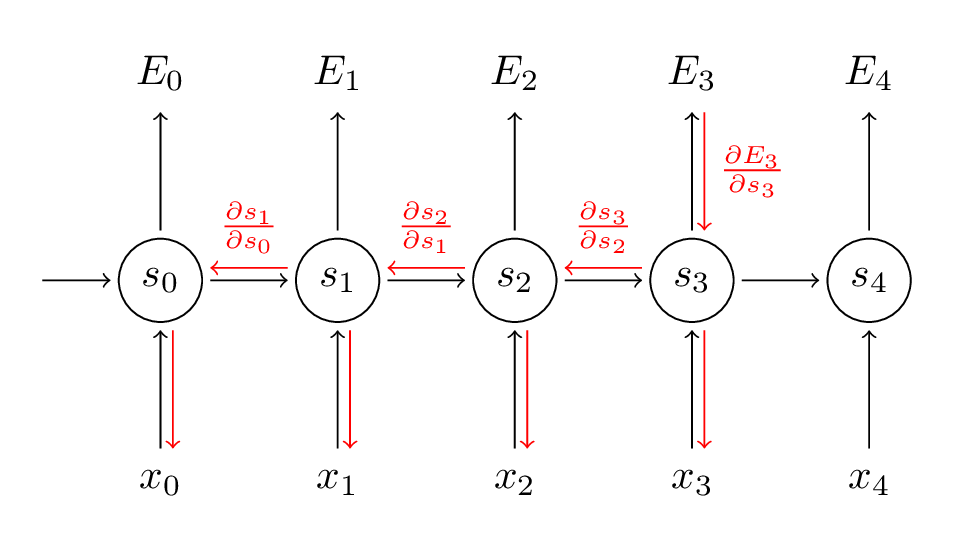
\includegraphics[width=\figwidth]{rnn-bptt-with-gradients}
	\caption[Backpropagation through time]{
		Backpropagation through time with gradients. Graphic is reproduced, extended by additional information and based on \textcite{Britz2015}.
		\label{fig:rnn-bptt-with-gradients}}
\end{figure}

The \textit{vanishing gradient effect} occurs since derivatives are repeatedly multiplied \cite{Skansi2018}. 
If a gradient's predecessors are equal or close to zero, the gradient itself is very small and weights are hardly updated, resulting in hardly changing weights and limited learning in early layers \cite{Britz2015, Hochreiter1991, Lillicrap2019}.
\textcite{Pascanu2013} states that the vanishing gradient effect occurs 
"when long term components go exponentially fast to norm 0, 
making it impossible for the model to learn correlation between temporally distant events" (p. 2).

During an explosion of long term dependencies, where a sequence of gradients is larger than 1, the \textit{exploding gradient effect} occurs \cite{Pascanu2013}.
Here, during backpropagation, the gradient can grow exponentially with each layer \cite{Philipp2017, Hochreiter1997, Lillicrap2019}.
The \textit{learning step} can become too large, causing an instability in the learning \cite{Lillicrap2019} driving the model not closer to an optimum but further away \cite{Skansi2018},


\subsection{Long-short-term memory} \label{sec:LSTM}
Long-short-term memory (LSTM) networks, firstly proposed by \textcite{Hochreiter1997}, tackle the problem of vanishing and exploding gradient successfully \cite{Skansi2018}.
They are categorized as a special kind of \glspl{rnn} \cite{Hoffmann2017}, made up of several gates \figref{fig:LSTM-chain}, which control how information flows through the network \cite{Valipour2017}.
They have an input gate, a forget gate and an output gate which are able to learn \cite{Valipour2017} and control what information should be removed and what information should be added \cite{Skansi2018}.
This way, LSTMs are able to learn to detect \textit{long term dependencies} \cite{Chung2014}.

\begin{figure}[H]
	\centering
	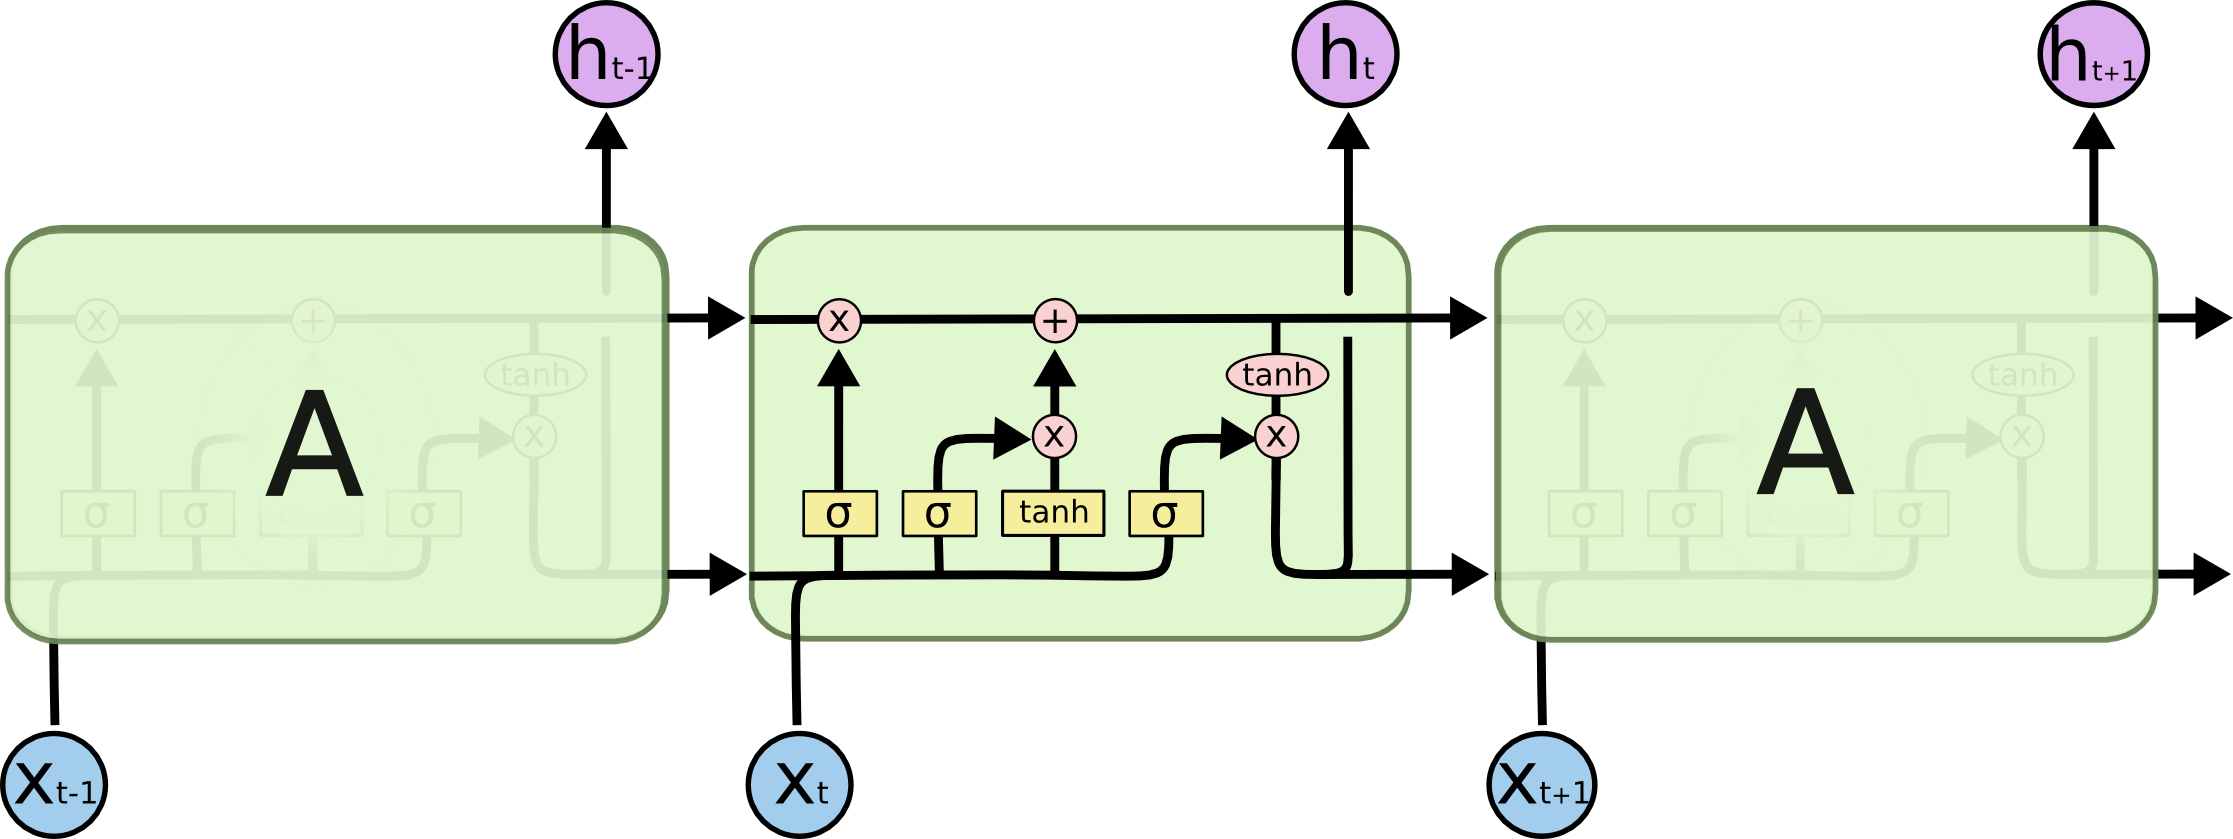
\includegraphics[width=\figwidth]{LSTM-chain}
	\caption[Long-Short-Term-Memory Architecture]{
		Long-Short-Term-Memory architecture. Graphic is reproduced and based on \textcite{Olah2015}.
		\label{fig:LSTM-chain}}
\end{figure}


\begin{equ}[!ht]
	\begin{equation}
		f_t = \sigma{(W_f * [h_{t-1},x_t] + b_f)} % Concatination?
	\end{equation}
	\begin{equation}
		i_t = \sigma{(W_i * [h_{t-1},x_t] + b_i)}
	\end{equation}
	\begin{equation}
		o_t = \sigma{(W_o * [h_{t-1},x_t] + b_o)}
	\end{equation}
	\begin{equation}
		\widetilde{C}_t = \tanh{(W_C * [h_{t-1},x_t] + b_C)} 
	\end{equation}
	\begin{equation}
		C_t= f_t * C_{t-1} + i_t * \widetilde{C}_t 
	\end{equation}
	\begin{equation}
		h_t = o_t * \tanh{(C_t)}
	\end{equation} 
\caption[LSTM Gates]{Formulas to compute the different gates and states. Extracted from \textcite{Chung2014} and \textcite{Hochreiter1997}} 
\label{equ:lstm}
\end{equ}

The LSTM network has, in addition to the \textit{hidden state}, a so-called \textit{memory cell} \cite{Hochreiter1997} or \textit{(internal) cell state} \cite{Valipour2017, Skansi2018, Lee2017, Yurdakul2017}.
$f_t$ denotes the output of the \textit{forget gate}, which is calculated by the hidden state from the previous timestep ($h_{t-1}$) and the current input $x_t$ at time point $t$ \cite{Lee2017}.
It controls how much of the input and the hidden state should be remembered \cite{Skansi2018}.
$i_t$ refers to the output of the \textit{input gate}, whose purpose is "to protect the memory contents stored (...) from perturbation by irrelevant inputs" (\cite{Hochreiter1997}, p. 6).
\textit{Candidate values} $\widetilde{C}_t$ are calculated and are combined with $i_t$ to update the cell state $C_t$ \cite{Hochreiter1997,Chung2014}.
The cell state $C_t$ is updated with each new input by the result of the forget gate $f_t$ and the result of $i_t * \widetilde{C}_t$ \cite{Chung2014}.
The different gates can be seen as \textit{filters} that determine which information will be saved in the cell state \cite{Skansi2018}.
Finally, the new hidden state $h_t$ is based on the result of the output gate $o_t$ combined with the new resulting cell state $C_t$.

Vanilla LSTMs are capable to process one dimensional sequential data through several gates and operations.
\textcite{Shi2015} proposed an extension of the fully connected LSTM by replacing multiplication operations in equations \ref{equ:lstm} with convolution operations, called a \gls{convlstm} \cite{Yurdakul2017, Nabavi2018}.
This way, the spatial information that might be incorporated in the data (\eg in images) will not get lost through any kind of dimension reduction that would have been necessary previously \cite{Shi2015}.
Their biggest advantage is that they are able to keep the dimensions of the input while reducing the necessary parameters \cite{Pfeuffer2_2019}.
Further research towards improving the \gls{convlstm} architecture has been done.
\textcite{Pfeuffer2_2019} proposed three alternations, namely \textit{Spatially Separable- , Depthwise- and Depthwise-Separable Convolutional LSTMs}, 
which reduced the number of parameters and operations while keeping a comparable performance like the original \gls{convlstm}  \cite{Pfeuffer2_2019}.

\subsection{Gated-Recurrent-Unit} \label{sec:GRU}
\textcite{Cho2014} proposed an alternative architecture that is able to learn long term dependencies using gates \cite{Chung2014}, the \gls{gru}.
The \gls{gru} architecture is similar to the LSTM architecture, but reduces the number of gates from three to two, namely an \textit{update-} $(z_t)$ and a \textit{reset gate} $(r_t)$ \cite{Dey2017} (see figure \ref{fig:GRU-chain}).
Moreover, the memory cell that was present in the LSTM is merged with the hidden state in the \gls{gru} \cite{Olah2015}.
The output flow of information is not controlled by an output gate, but is determined indirectly by the update- and reset gates that control the information of the hidden state \cite{Siam2018}.

\begin{figure}[H]
	\centering
	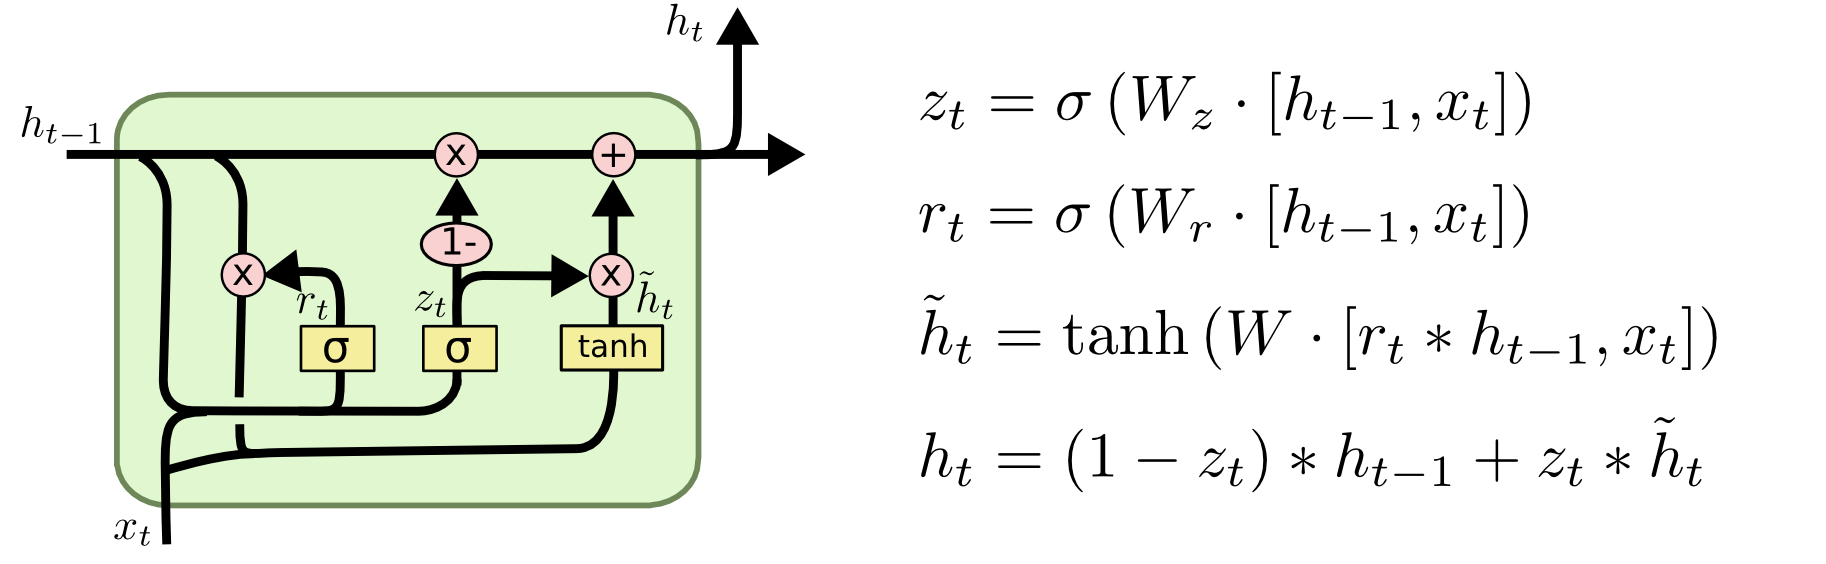
\includegraphics[width=\figwidth]{GRU-chain}
	\caption[Gated-Recurrent-Unit Architecture]{
		Gated-Recurrent-Unit architecture. Graphic is reproduced and based on \textcite{Olah2015}.
		\label{fig:GRU-chain}}
\end{figure}


\begin{equ}[!ht]
	\begin{equation}
		z_t = \sigma{(W_z * [h_{t-1},x_t])} % Concatination?
	\end{equation}
	\begin{equation}
		r_t = \sigma{(W_r * [h_{t-1},x_t])}
	\end{equation}
	\begin{equation}
		\widetilde{h}_t = \tanh{(W * [r_t*h_{t-1},x_t])} 
	\end{equation}
	\begin{equation}
		h_t = (1-z_t)*h_{t-1}+z_t*\widetilde{h}_t
	\end{equation} 
\caption[GRU Gates]{Formulas to compute the different gates and states. Extracted from \textcite{Chung2014}}
\label{equ:gru}
\end{equ}

Less gates that modulate the information flow in fewer states \cite{Chung2014} leads to a simpler architecture that is faster to train \cite{Yurdakul2017} and consumes less memory \cite{Valipour2017}.
While both, LSTMs and \glspl{gru}, outperform classical \glspl{rnn} in tasks that require long-term dependencies \cite{Chung2014}, \glspl{gru} show a similar good performance to the LSTM architecture while having a reduced complexity \cite{Valipour2017}.
\textcite{Dey2017} argue that \glspl{gru} outperform LSTMs in most cases. 
\textcite{Jozefowicz2015} confirm this observation with the restriction that LSTMs outperform \glspl{gru} in language modelling tasks.

In order to process two-dimensional data, \glspl{convgru} have been designed \cite{Ballas2016,Siam2018}.
Dot product operations in the classical \gls{gru} formulas (see equations \ref{equ:gru}) are replaced by two dimensional convolution operations \cite{Siam2018} and states and gates are three dimensional tensors \cite{Tokmakov2017}.

\section{Related Work} \label{sec:related_work}

\subsection{Semantic Segmentation Architectures}\label{sec:SemanticSegmentation}

Segmenting an image into its individual parts is a classical problem of computer vision \cite{Szeliski2011}. 
Early approaches involve typical methods like threshold detection \cite{Smith1979}.
More modern approaches like k-means clustering \cite{Dhanachandra2015} improved the early results.
Deep learning architectures, especially \glspl{cnn} \cite{Fukushima1980}, have lead to further improvement \cite{Minaee2020}.
\textcite{Shelhamer2014} have been the first to propose a \gls{cnn} architecture where a pixel-wise supervised training was achieved. 
This was done by upsampling the class prediction layer to the input image size, leading to an end-to-end pixel-wise classification, a \textit{Fully Convolutional Network} \cite{Shelhamer2014}.
Following papers proposed different architectures.
A \textit{Deconvolutional Network} with special unpooling and deconvolution operations was invented by \textcite{Noh2015}. 
Here, the information was enconded using several convolution and pooling layers and was decoded using unpooling and deconvolution.
The \textit{SegNet} model uses a similar Encoder-Decoder architecture by using pooling indices to upsample the image to its original size after encoding \cite{Badrinarayanan2017}.
\textit{ICNet} was able to perform semantic segmentation not only in real-time, but also for high quality images (1024x2048 at 30 fps) \cite{Zhao2017}. 
This was achieved by using a cascade image input of different resolutions. 
The authors made use of the semantic information from the scaled down images and the details from the high resolution images.
In this way, they have been able to achieve a "trade-off between efficiency and accuracy" (\cite{Zhao2017}, p.2).
Google's approach towards instance segmentation is called DeepLab and has evolved over the last recent years.
The first DeepLab version uses a combination of Deep \glspl{cnn} with fully connected \glspl{crf} \cite{Lafferty1999} that try to grasp the semantic context of the image \cite{Chen2016}. 
One of their contributions is the use of \textit{atrous-} (also called \textit{dilated-}) convolutions as an alternative to deconvolution \cite{Chen2016}.
Originally used for wavelet transformations \cite{Mallat1999}, a new parameter \textit{r} allows to change the stride at which the samples are taken during the convolution operation \cite{Chen2016}. (3x hintereinander gleiche quelle, zusammenfassen? TODO)
Applying dilatation during convolution allows to increase the receptive field while keeping the computational costs low \cite{Minaee2020}.
This approach has been further improved and \Gls{aspp} \figref{fig:ASPP} has been introduced, which was based on the idea of combining atrous convolutions with spatial pyramid pooling (firstly introduced by \textcite{He2014}) \cite{Chen2018}.

\begin{figure}[H]
	\centering
	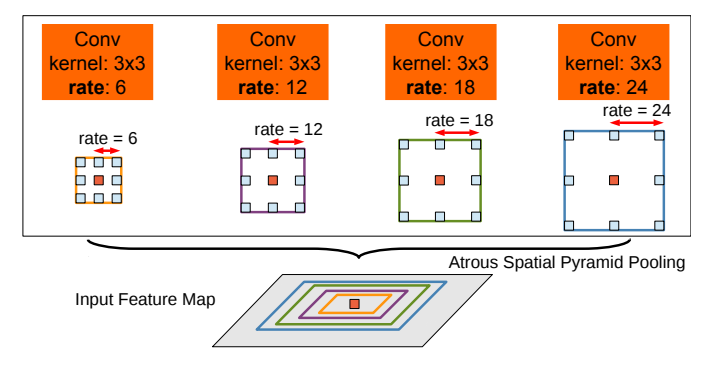
\includegraphics[width=\figwidth]{ASPP}
	\caption[Atrous Spatial Pyramid Pooling]{
		Atrous Spatial Pyramid Pooling. (\cite{Chen2018}, Fig. 4).
		\label{fig:ASPP}}
\end{figure}


In \gls{aspp}, parallel filters of different dilatation rates are concatenated with the intend to cover different field-of-views \cite{Chen2018}, allowing robust object segmentation on different scales \cite{Minaee2020}.
The most recent approach, DeepLab V3+, has an Encoder-Decoder structure and was able to show "new state-of-the-art performance on PASCAL VOC 2012 and Cityscapes datasets." (\cite{Chen2018b}, p.14).
The encoder is based on their previous DeepLabV3 architecture with a modified Xception backbone \cite{Minaee2020}.
The newly introduced decoder is responsible for upsampling the output to the desired size.
This is achieved by concatenating the encoders output after the \Gls{aspp} layers with the images' \textit{low-level features} that are extraced from backbone early layers, see figure \ref{fig:DLPlus} for the detailed architecture \cite{Chen2018b}.
More on the networks architecture can be found in section \ref{sec:Architecture}.
Moreover, the Google research team has shown that they are able to create an Encoder-Decoder architecture that is very light and fast.
This architecture is light enough to run at real-time on modern smartphones \cite{Bazarevsky2018}.

\begin{figure}[H]
	\centering
	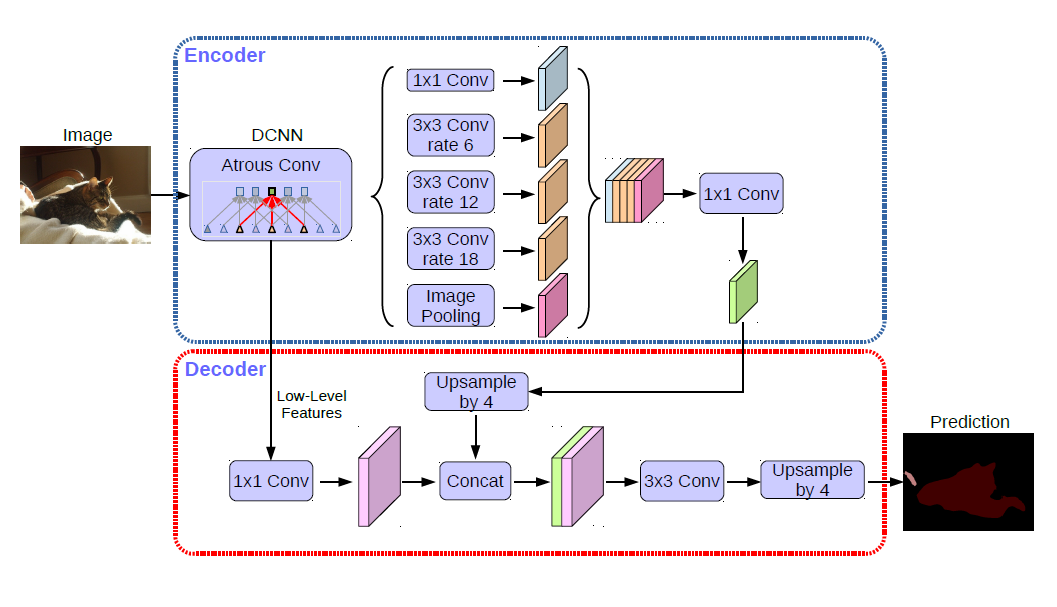
\includegraphics[width=\figwidth]{DLV3Plus}
	\caption[DeepLabV3+ Architecture]{
		DeepLabV3+ Encoder-Decoder Architecture \cite{Chen2018b}.
		\label{fig:DLPlus}}
\end{figure}


\subsection{Video processing}

The segmentation models in section \ref{sec:SemanticSegmentation} are usually evaluated on individual images.
However, in real world scenarios segmentation for videos is often necessary and not just single images.
Naturally, the segmentation works on each individual frame, but this way the temporal information of the videos that is present in the image sequence gets lost \cite{Garcia-Garcia2018}.
A network that evaluates each frame independently is not able to know that the previous frame is related to the current one and treats each frame independently \cite{Pfeuffer2019}.

Extending existing models with a \gls{ru} could enable the model to not only use spatial but also temporal information \cite{Pfeuffer2019}.
As mentioned in section \ref{ch:RNN}, \glspl{rnn} are usually the answer to time dependent problems \cite{Hoffmann2017} or used for sequential data such as in time series analysis or text translation. 
\textcite{Valipour2017} were one of the first to introduce a \gls{ru} into a segmentation model \cite{Pfeuffer2019}, increasing the models performance by 3 - 5\%.
\textcite{Visin2015} introduced ReSeg, a segmentation model consisting of four \gls{rnn} layers that "sweep the image horizontally and vertically" (p.1).
\textcite{Yurdakul2017} was also able to improve performance by incorporating \glspl{convlstm} (\ref{sec:LSTM}) and \glspl{convgru} (\ref{sec:GRU}) in their architecture.
% positions of the RU
The positioning of the \gls{ru} in existing models varies across the literature.
\textcite{Pfeuffer2019} note that \glspl{ru} are often placed between of the encoder and decoder, for example as in \cite{Valipour2017,Yurdakul2017}.
\textcite{Pfeuffer2019} investigated the effect of the placement of a \gls{convlstm} cell on the performance of the model and observed that the best position for \gls{convlstm} layer seems to be directly in front of the last activation layer and not in between the encoder and decoder \cite{Pfeuffer2019}.
In their follow up work \cite{Pfeuffer2_2019}, different \gls{convlstm} variations have been investigated with the intend to lower the complexity and allow for faster video segmentation.

\chapter{Methods} 
\label{ch:Methods}


\section{The Dataset}\label{sec:Dataset}
\subsection{Requirements}\label{sec:Requirements}
The task of a binary semantic segmentation in this work upholds certain requirements towards the dataset that is used for training.
The dataset should have two classes, one foreground and one background class.
The model input frames should be in a typicial 3-channel format with \gls{rgb} channel values in the range of 0 to 255 (normalized to 0 and 1). 
The ground truth needs to be in a typical 1-channel greyscale format where each pixel is either black or white, representing the background and foreground class respectively.
Since the model is supposed to use temporal information through a \gls{ru}, the images need to be the individual frames from a video file in the order they occur, they are not randomized within one video.
The content of the video should be focused around human beings in the foreground, since the use case scenario of the network is a background replacement task of humans in a convention/event scenario.
In addition to that, it is required that the dataset is flexible in terms of the background.
As mentioned, the backgrounds in the input image that the model is supposed to remove are expected to be designed based on the individual customer.
The specific design is known prior to the models use, which means the dataset should support the possibility to train the model for a specific background in order to improve and overfit the model to some extend towards certain prior given backgrounds.

The final dataset is separated into a training and testing set.
The training set consists of 74852 CHECK images and labels while the testing dataset consist of 20280 CHECK images and labels, corresponding to a 78 to 22 CHECK train-test-ratio.

\subsection{Creating the Dataset}
These requirements are very specific and to the best of our knowledge, there is no dataset that would fullfill the given requirements.
Therefore, this thesis proposes a newly crafted dataset that is able to fullfill all requirements described in \ref{sec:Requirements}.
The \gls{gt} images (or \textit{labels}) based on the video input frames are produced in an automatic manner (see \ref{sec:Preprocessing} for details) using a colour threshold algorithm.
Creating high quality \gls{gt} images by hand is a very laborious work and simply too time consuming considering that individual video frames need to be labeled.
A selection of 70 publicly available greenscreen stock video clips, varying in length from 4 seconds to 3:06 minutes, is used as the basis for the training dataset.
The testing dataset is based on one large video of length 11:18 minutes.
The testing dataset video is completly different from the training dataset, meaning that no person that can be seen in the training dataset is also present in the testing dataset.
The background of those clips is replaced by one of 160 background images, which have been randomly separated into 128 training and 32 testing backgrounds to ensure no overlap between the training and testing dataset.
The selection of the background images is based on certain criteria.
Looking at various existing background walls that are used by companies for presentation on conventions one can observe that their designs are usally quite similar.
The overall design is centered around the product of the company, the companies logo, is usually kept very minimalistic with some basic geometric shapes, abstract with some chaotic or repetitive patterns or has a nature like theme.
In addition to that, letters are likely to appear referring to the companies name or commercial slogan.
Based on these criteria the selection of background images has been made.

\section{Preprocessing}\label{sec:Preprocessing}
Several preprocessing steps have been done to prepare the data into a format suitable for training.
The raw greenscreen video clips are separated into four seconds snippets and scaled down by a factor of four to a resolution of 270x512 pixels.
The resulting clips are randomly shuffled and the green background is replaced by one randomly selected background image out of the pool of background images for each of the four seconds clips.
In order to prevent potential overfitting and to increase the data variation random data augmentation has been added to the training loop.
These augmentations are applied to each frame (input and label) that belong to the same four seconds video clip.
With the start of each new four seconds video the amount of augmentation is determined again.
Each of the following augmentations is applied with a probability of 50\%:CHECK
- frames are horizontally flipped.
- frames are rotated randomly by a random degree with a maximum rotation of 10 degrees and a minimum degree of -10 degree. % the image will be scaled by a factor.
- frames are translated into x and y direction by a random value in the range of -10 to 10.
- frames are transformed by the \textit{shear effect} TODO by a factor in the range of -7 to 7.
- the input frames brightness is adjust by a factor of 0.6, 0.8, 1.2 or 1.4.

Moreover, if an image is rotated or translated it is also sclaed by a factor of 1, 1.1, 1.2 or 1.3 randomly.
Lastly, the images are normalized based on the ImageNet mean ([Red: 0.485, Green: 0.456, Blue: 0.406]) and standard deviations ([0.229, 0.224, 0.225]) TODO QUELLE TODO.
The reason for this is that the backbone of the DeepLabs is pretrained on the ImageNet dataset TODO QUELLE TODO.


\section{Network Architecture} \label{sec:Architecture}
The DeepLabV3+ architecture that was briefly touched upon in \ref{sec:SemanticSegmentation} will be working as a basis for the final model architecture.
Its components can be broken down into two parts, the backbone and the classifier.
The backbone is a pretrained network from which intermediate results are extracted and fed into the classifier.
The classifier is separated into an encoder and a decoder part.
The encoder receives high-level features from later layers of the backbone (layers 5-18) while the decoder receives low-level features from early layers of the backbone (layers 1-4).
\textcite{Chen2018b} have investigated the influence of different backbones that are pretrained on different datasets.
For example, they showed that using an Xception network \cite{Chollet2017} over a Resnet-101 \cite{He2016} (both pretrained on the ImageNet-1k dataset \cite{Russakovsky2015}) improves the models performance.
Further training on datasets like the MS-COCO \cite{Lin2014} yielded a further improvment by 2\%.
Since the backbone does seem to have an effect on the network performance, two different pretrained backbones will be compared.
A Resnet-50 as described by \textcite{He2016} and a MobileNetV2 \cite{Sandler2018} to see if the changes of the network are dependent on the backbone.
This thesis will further refer to the DeepLabV3+ as the \textit{base model}.

\subsection{Adding Recurrency} \label{sec:AddingRecurrency}
Several different alternations have been made to the base model to investigate the effects of \gls{ru} on the networks performance.
In this work two different positions for \glspl{ru} are investigated.

\begin{figure}[H]
	\centering
	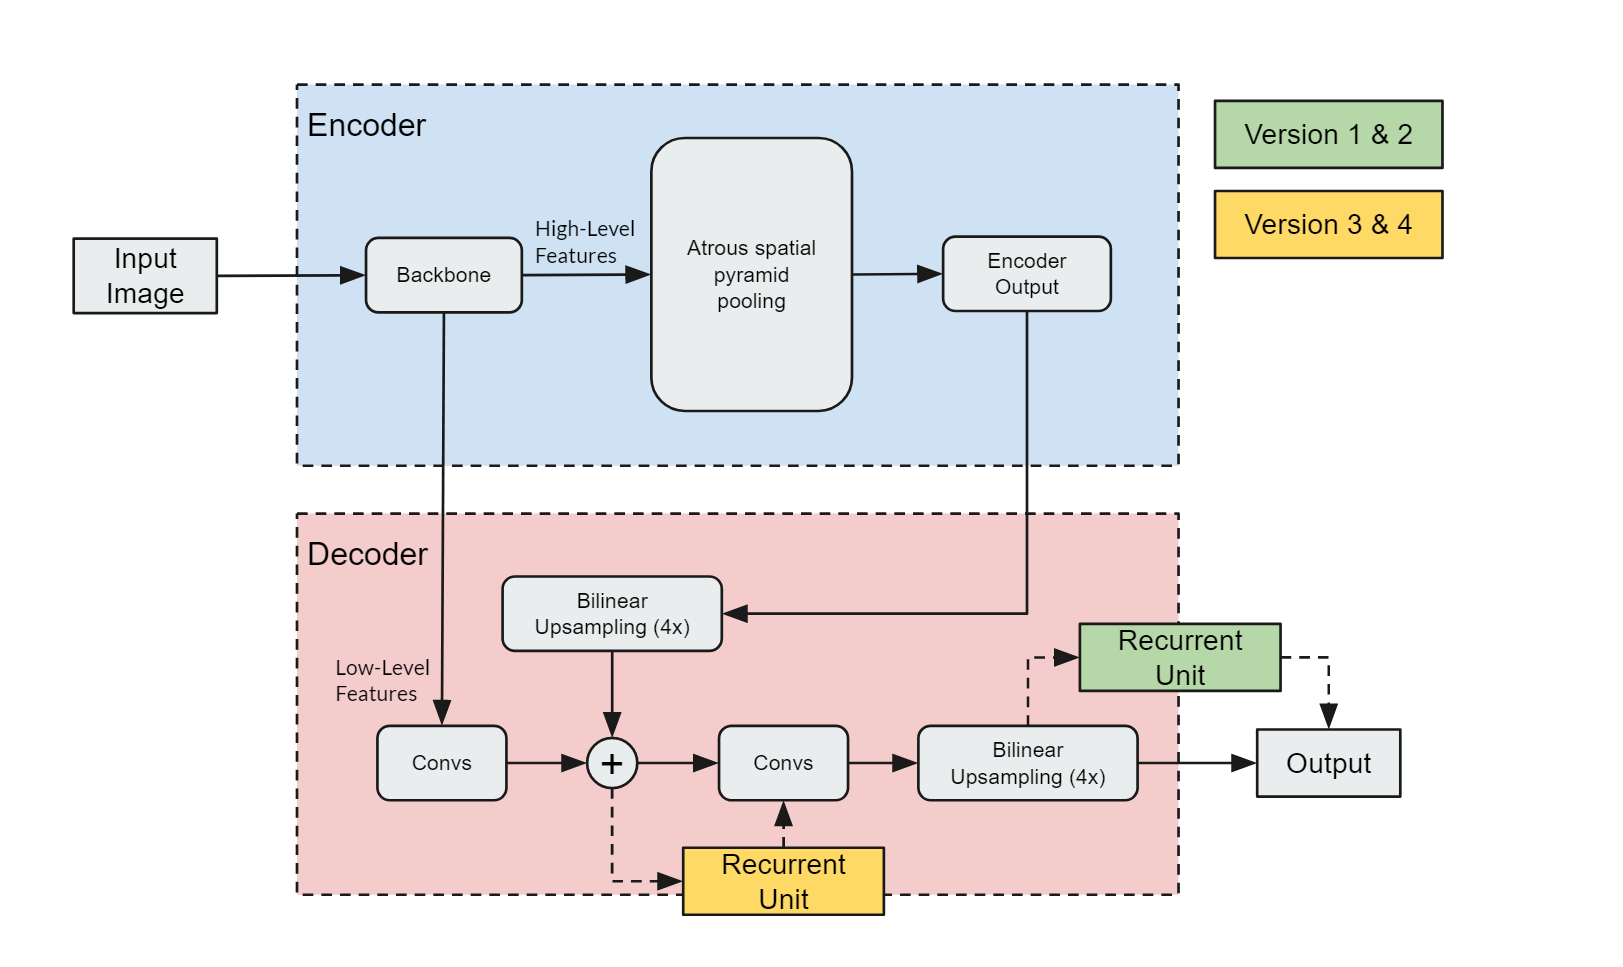
\includegraphics[width=\figwidth]{DLV3Plus_RU}
	\caption[DeepLabV3+ Architecture with Reccurent Units]{
		DeepLabV3+ Encoder-Decoder Architecture with additional recurrent units.
		\label{fig:DLPlus}}
\end{figure}

Network version 1 is the base model but with one additional \gls{ru} at the end of the segmentation, before the last activation function.
Version 3 is the base model but with one additional \gls{ru} after the concatination of the encoders output and the processed low-level-features.

In addition to that this work investigates if varying the amount of previous timestep results that are fed into the \gls{ru} will help the network to segment the image.
To be precise, either one timestep after the other is fed into the \gls{ru} or two previous timesteps are fed into the \gls{ru}.
In both scenarios the hidden state (and cell state for the LSTM) are kept in between the individual batches as long as they belong to the same video.
Network version 2 is equal to version 1, but while version 1 only receives the current timestep $[t]$, version 2 receives the output of the previous two timesteps $[t-2,t-1,t]$.
Version 4 of the network is equal in structure to version 3 but will also receive the output of the two previous timeframes.

In total, this work investigates the base model and its 4 different versions described above.
In addition, two different \glspl{ru} are investigated (\glspl{convlstm} and \glspl{convgru}) and two different backbones (Resnet-50 and MobileNetV2).
This gives a total of 5x2x2 TODO possibilities and 20 different networks to compare.
Combinations of different positions of the \glspl{ru} are not investigated since the experiments by \textcite{Pfeuffer2019} suggest that this does not improve perfomance.

The two additional timesteps that fed into the \glspl{ru} can be seen as an additional dimension.
The tensors are therefore translated from a shape of [batch size, number of channels, heigth, width] into [batch size, timesteps, number of channels, heigth, width] with the timestep dimension being 1 in case of version 1 and 3 and being 3 in case of version 2 and 4.
Internally, the individual timesteps are processed by the \glspl{ru} in a loop-like manner, starting with oldest timestep $t-2$.
The output of the \glspl{ru} is of same shape as the input with an extra timestep dimension.
%TODO ANFANG% Eventuel rausnehmen/umschreiben, falls kein 1x1 conv3d mehr da ist 
However, in order for the network to process the output of the \glspl{ru} even further, this additional dimensionality needs to be removed.
This is done by a 1x1 pointwise convolution along the \textit{timestep dimension} as similiarly described in \cite{Sandler2018} and also used by \cite{Chen2018b}.
This way the number of timestep feature is reduced from three to one without lossing information.
%TODO ENDE% 


\section{Training}
The training of the models is performed on the \textit{Grid-Computing-Network} of the Institute of Cognitive Science Osnabrück.
This allowed to train multiple models simultaniously on modern graphic cards. Evaluation has been performed on NVIDIA GTX 1080Ti TODO REFERENCE

TODO weitere system details TODO

\subsection{Implementation Details}
All networks are implemented in python version 3.6.10 with pytorch <TODO>Version<TODO> as the main library to implement the neural networks.
As an optimizer Adam \cite{Kingma2015} was chosen, which is more suitable for \glspl{rnn} than others such as \textit{Stochastic Gradient Descent} \cite{Pfeuffer2020}.
Hyperparameters such as \gls{wd} and \gls{lr} are changed for each model, see \ref{sec:Hyperparameters} for a detailed explanation on how the values are determined.
As a \gls{lr} scheduler strategy a cyclic learning rate has been used.
The "triangular2" (\cite{Smith2017}, p.3) strategy lets the \gls{lr} cycle in between a predefined lower and upper \glspl{lr}, with the additional effect of reducing the cycle range into half after each cycle \figref{fig:LRscheduler}.
The length of one cycle is based on the parameter \textit{stepsize} (or "number of iterations in one epoch" (\cite{Smith2017}, p.3)) is calculated by dividing the length of the dataset by the batch size.

\begin{comment}
\begin{figure}[H]
	\centering
	\includegraphics[width=\figwidth]{TODO}
	\slcaption{
		triangular2 \gls{lr} scheduler strategy with a stepsize of TODO.
		\label{fig:LRscheduler}}
\end{figure}
\end{comment}

As a loss function the dice similiarity coefficient has been choosen, which is next to the categorical cross entropy one of the most common loss functions for semantic segmentation \cite{Garcia-Garcia2018}.
Using the dice coefficient as a loss function has been proposed by \textcite{Milletari2016}.
For N total pixels, p denoting the prediction and g refering to the ground truth, the dice loss is defined as \cite{Milletari2016}:
\begin{equ}[H]
	\begin{equation}
		\text{Dice loss} = 1 - \frac{2\sum_{i}^{N}p_i*g_i}{\sum_{i}^{N}p_i^2 + \sum_{i}^{N}g_i^2}
	\end{equation}
	\caption[Dice Loss]{Dice loss based on \textcite{Milletari2016}}
\end{equ}

\subsection{Hyperparameter Optimization} \label{sec:Hyperparameters}
During first initial training tests (\gls{wd}=0 and \gls{lr}=0.001) it was observable that some models loss convereged after a few epochs while other models loss diverged or was stuck in a local minima.
In order to ensure the models' convergence suitable hyperparameter need to be chosen for the individual models.
The \textit{Learning rate range test} (LR range test) was taken to systematically find model specific parameters.
This methodology is based on the work of \textcite{Smith2017}.
Firstly, an upper and lower learning rate has to be defined which will be the range of learning rates that will be investigated.
Secondly, the network will be trained and the learning rate will be increased exponentially after each individual training batch.
Lastly, the loss and the learning rate are recorded and plotted after training for 1 to N epochs \cite{Smith2017}.
The resulting learning rate vs. loss plot shows for which \gls{lr} values the loss does not change (lr is too small), for which the loss decreases (lr is just right) and for which the loss divereges (lr is too high).
This algorithm can be applied multiple times with different hyperparameter values in order to compare which values are most suited for the specific model on the specific dataset.

In his follow up work \textcite{Smith2018} investigates the batch size and weight decay in conjungtion with the \gls{lr} range test.
In terms of the batch size Smith concludes that one should pick the batch size that enables the highest learning rate but most importantly fits in the \gls{gpu} memory \cite{Smith2018}. 
To find the best suited \gls{wd} value the author also suggest a \gls{lr} range test for multiple \gls{wd} values.
However, the author also notes that in general it seems to be the case that smaller datasets require larger \gls{wd} values while larger datasets seem have a regularization effect on their own and therefore require small \gls{wd} values.
This argument is also supported by \textcite{Hernandez-Garcia2018} who showed that data augmentation (and therefore artificially increasing the dataset) has a similiar regularization effect on the model as weight decay, indicating that large datasets do not require further regularization through weight decay.

\begin{comment}
\begin{figure}[H]
	\centering
	\includegraphics[width=\figwidth]{}
	\slcaption{
		Batch size LR range test for model: TODO.
		\label{fig:BSLRtest}}
\end{figure}
\end{comment}

A \gls{lr} range test has been performed for multiple batch sizes for each model version described in section \ref{sec:AddingRecurrency}.
TODO shows the results of an example \gls{lr} range test.
In order to ensure that hardware resources are not exceeded and ensure comparability across all models a batch size of 8 was chosen for all models. 

With regard to the \gls{wd} hyperparameter, 4 different \gls{wd} values have been investigated with the \gls{lr} range test for each model as described by \textcite{Smith2018}.


\begin{figure}[H]
	\centering
	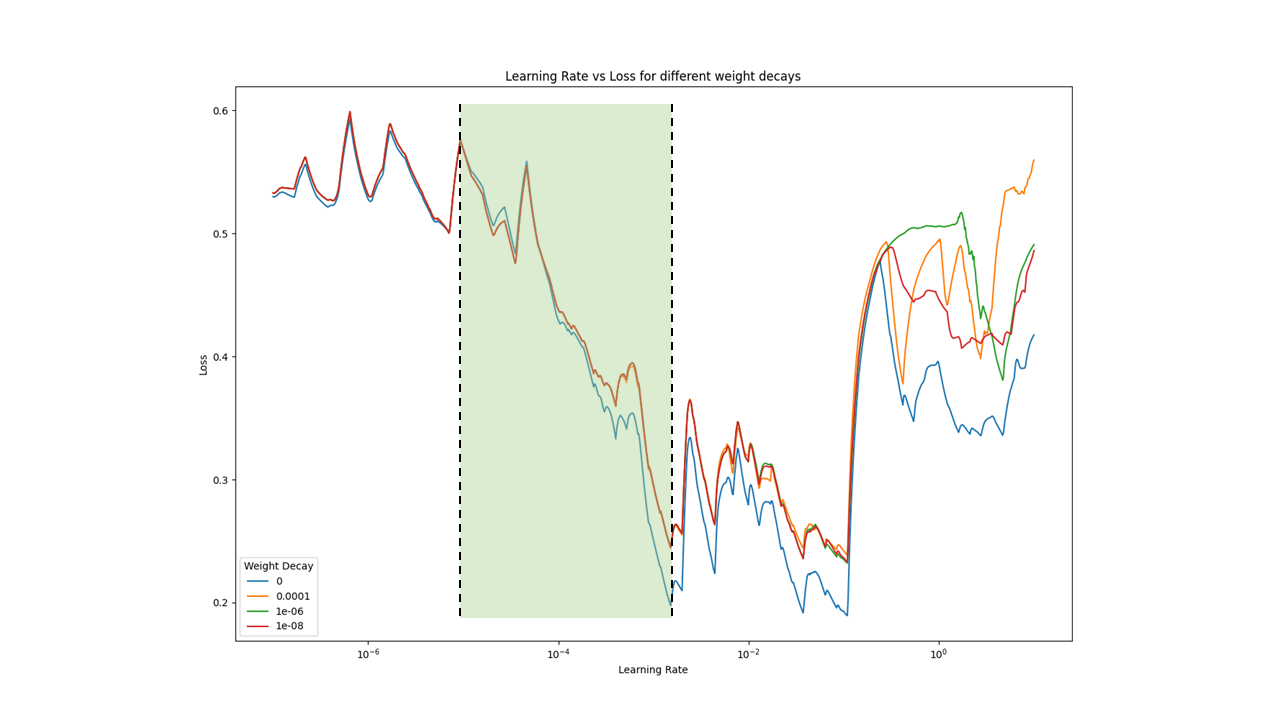
\includegraphics[width=\figwidth]{LR_plot_res_lstm_v2}
	\caption[Weight decay learning rate range test]{
		Weigh decay LR range test for base model + lstm version 2 with a Resnet-50 backbone.
		\label{fig:WDLRtest}}
\end{figure}


\figref{fig:WDLRtest} shows an exemplar \gls{lr} range test for different \gls{wd} values.
It can be seen how for \gls{wd}=0 the loss curve reaches the overall lowest point.
In contrast, a \gls{wd} of 1e-8 shows that their lowest point is higher than for \gls{wd}=0, therefore, a \gls{wd} value of 0 is prefered over the other \gls{wd} values.
What could be observed across all models is that low \gls{wd} values such as 0 or 1e-8 seem to achieve lower loss values.
This observation confirms the observations made by \textcite{Hernandez-Garcia2018} that for large datasets who apply data augmentation, which is present in this case, further regularization through weight decay is hardly necessary.
The lower \gls{lr} bound for the triangular2 \gls{lr} scheduler strategy should be the \gls{lr} value where the loss curve starts to fall and is not flat anymore.
For lower \glspl{lr} than the lower \gls{lr} bound the learning steps are too small to elicit a change in the loss function, hence, the lower \gls{lr} bound is the minimal \gls{lr} value where noticeable learning occurs \cite{Smith2018}.
The upper \gls{lr} should be picked in such a way that its loss is as low as possible while the \gls{lr} as high as possible, in the best scenario right before the loss increases rapidly which indicates divergence.
In the figure \ref{fig:WDLRtest} the green area marks the \gls{lr} range with the lower \gls{lr} bound 0.00001 and the upper \gls{lr} bound 0.001.
Although the loss is very low around 0.1, the loss fluctuates a lot in between 0.001 and 0.1.
During our initial experiments with a lr-range that includes the area of fluctuation it could be observed that the loss function had a tendency to diverge or get stuck in a local minima and did not change. TODO(bild raussuchen oder ggf. neu erstellen, falls nichtmehr vorhanden)


All \gls{wd} and \gls{lr} bound values for all models can be found in table TODO.
TODO: All \gls{lr} range test plots for the different models can be found in section TODO.
For some model version a \gls{wd} value of 1e-4 or 1e-6 immediatly diverged an is therefore not displayed in some of the plots.

\section{Metrics}

(TODO Formeln weglassen? Weniger Metricen? auf eine formulierungsart festlegen?)

In order to evaluate the different models objective meassurements are required that allow for a fair comparison across multiple models \cite{Garcia-Garcia2018}. 
\textcite{Minaee2020} and \textcite{Garcia-Garcia2018} nicely summarize the most common metrices used for semantic segmentation.

The \gls{pa} is defined as the ratio of correctly classified pixels to the total number of pixels:
\gls{tp} denotes the pixels correctly classified as the class of interest, 
\gls{tn} denotes the pixels correctly classified as not the class of interest, 
\gls{fn} denotes the pixels that are classified as not the class of interest while actually belonging to class of interest and lastly
\gls{fp} denotes the pixels that are classified as class of interest while actually not belonging class of interest.
The classes of interest are in our binary context the foreground and the background class.

\begin{equation}
	\text{PA} = \frac{(\TP + \TN)}{(\TP + \TN + \FP + \FN)}
\end{equation}

In a more general context, for $k + 1$ classes and pixel $p_{ij}$ denoting the pixel of class i classified as belonging to class j, the pixel accuracy can be described as \cite{Garcia-Garcia2018}:

\begin{equation}
	\text{PA} = \frac{\sum_{i=0}^{k}p_{ii}}{\sum_{i=0}^{k}\sum_{j=0}^{k}p_{ij}}
\end{equation}

The \gls{mpa} calculates the pixel accuracy for each class and avereges over the total number of classes:

\begin{equation}
	\text{MPA} = \frac{1}{k+1}\sum_{i=0}^{k}\frac{p_{ii}}{\sum_{j=0}^{k}p_{ij}}
\end{equation}


The most frequently used metric in semantic segmentation is the \gls{iou} (or \textit{Jaccard Index}) \cite{Minaee2020}.
It computes the area of overlap of the ground truth and the prediction divided by the union of both areas \cite{Garcia-Garcia2018}:

\begin{equation}
	\text{IoU} = \frac{\TP}{(\TP + \FP + \FN)}
\end{equation}


The \gls{miou} computes the average of the per class calculated \glspl{iou} \cite{Garcia-Garcia2018}:

\begin{equation}
	\text{Mean IoU} = \frac{1}{k+1} \sum_{i=0}^{k} \frac{p_{ii}}{\sum_{j=0}^{k} p_{ij} + \sum_{j=0}^{k} p_{ji}-p_{ii}}
\end{equation}

Lastly, a popular metric is the Dice Score, which is in our boolean context equivialent to the F1 score \cite{Minaee2020}. It is defined as: TODO Kursiv?

\begin{equation}
	\text{Dice}=\frac{2\TP}{2 \TP + \FP+ \FN}
\end{equation}

TODO MEAN DICE?
The \gls{miou} and Dice score heavily penalize missclassifications.
Consider a \gls{gt} image that is mostly background with one foreground pixel.
If this foreground pixel is not predicted correctly, while the background is mostly correct predicted,
the number of \gls{tp} is 0, which means the whole metric value for the foreground class is 0.
For the background class this value would be close to 1.
Ultimately, the average is taken over our 2 classes which results in a metric value close to 0.5, even though one class is predicted almost perfectly.

\chapter{Results}

\begin{table}[ht]
	\addtolength{\leftskip} {-2cm}
    \addtolength{\rightskip}{-2cm}
	\begin{tabular*}{1.2\textwidth}{@{\extracolsep{\fill}}|l|r|r|r|r|r|r|r|r|}
	\toprule

	\renewcommand\arraystretch{1}
	Metric & \multicolumn{2}{c|}{Mean IoU (\%)} & \multicolumn{2}{c|}{Dice(\%)}&  \multicolumn{2}{c|}{\vtop{\hbox{\strut Pixel}\hbox{\strut Accuracy(\%)}}} & \multicolumn{2}{c|}{\vtop{\hbox{\strut Per Class}\hbox{\strut Accuracy(\%)}}} \\
	\midrule
	Dataset &    					Train &    Validation 	  &  	Train &    Validation 	&Train &    Validation & Train &    Validation \\
	\midrule	
	base          	&   			 68.69 & 			51.64 &  	79.05 &  58.22 & 89.58 &  87.15 & 92.49 &  80.09 \\
	+ GRUV1  		&   			 52.61 &   \textbf{63.47} &  	61.31 &  71.30 & 84.43 &  90.83 & 90.60 &  85.59 \\
	+ GRUV2  		&   			 56.76 & 			55.09 &  	67.42 &  61.76 & 84.11 &  87.96 & 90.72 &  86.08 \\
	+ GRUV3  		&   			 68.37 & 			61.23 &  	77.20 &  70.66 & 88.32 &  86.25 & 81.02 &  72.77 \\
	+ GRUV4  		&   	\textbf{81.49} & 			60.34 &  	89.03 &  70.54 & 91.93 &  82.05 & 89.12 &  71.25 \\
	+ LSTMV1 		&    	\textbf{39.62} &  \textbf{66.20}  &  	46.26 &  74.54 & 76.00 &  89.71 & 76.90 &  76.95 \\
	+ LSTMV2 		&   			 74.75 &  \textbf{69.37}  &  	84.36 &  77.38 & 89.09 &  90.66 & 87.74 &  79.51 \\
	+ LSTMV3 		&   	\textbf{90.22} &  			68.12 &  	94.58 &  76.75 & 95.96 &  89.42 & 95.34 &  79.87 \\
	+ LSTMV4 		&   			 67.58 &  			65.43 &  	77.77 &  72.87 & 86.93 &  90.68 & 85.38 &  83.81 \\
	\bottomrule
	\end{tabular*}
\end{table}

Highest \gls{miou} on train is \gls{lstm} Version 3 with 90 \%, while on the validation dataset the \gls{lstm} version 2 and 3 perfome better

\chapter{Evaluation and Discussion} 

\section{Complexity}\label{sec:complexity}
It is important to consider the complexity increase when making alternations to existing models.
One has to evaluate whether the complexity increase of the model is justified by the increased performance.
In order to evaluate the increased complexity of the different network versions two factors are investigated, the \textit{Inference time} and the \textit{Number of model Parameters}.
The inference time in this work is meassured by the time (in \gls{ms}) it takes the network to make a predict on a single frame and the application of argmax to extract the class predicitons for each pixel.
Assuming that a framerate of 25 frames per seconds would mean \textit{real-time performance}, a network need to be able to predict one image within 25 \gls{ms} to achive real-time perfomance.
The number of model parameters refers to the number of weights and biases a network architecture has, the higher the number of parameters, the \textit{deeper} and more complex the network is.
This way we can compare the size and the prediction speed of the models.


\begin{figure}[H]
	\centering
	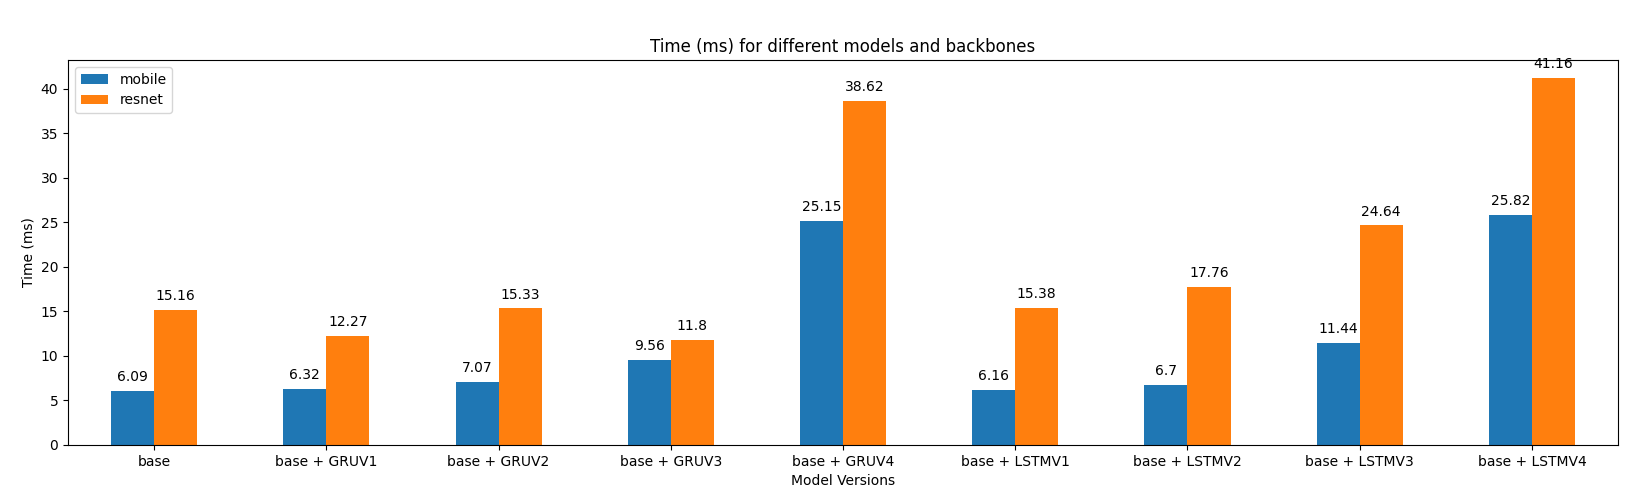
\includegraphics[width=\figwidth]{time_results}
	\caption[Inference Time Results]{
		Evaluation of the inference time (in \gls{ms} of the different model versions for the different bacbkones (MobileNetV2 and Resnet-50).  
		\label{fig:Inference_time}}
\end{figure}
TODO (Tabelle auch einbringen?)

\begin{table}[ht]
	\centering
	\renewcommand\arraystretch{1.2}
	\begin{tabular}{|l||r|r|r|r|c|}
		\toprule
		{Backbone} 				& \multicolumn{2}{l|}{Mobile} 	& 									\multicolumn{2}{l|}{Resnet 50} 										&Absolute\\ %\multirow{2}{*}{Absolute increase}
		\cmidrule{1-5}
		Number of Parameters 	& \multicolumn{1}{c|}{Absolute} & \multicolumn{1}{c|}{Percentage} &	\multicolumn{1}{c|}{Absolute} 	&	\multicolumn{1}{c|}{Percentage} &increase\\
		\midrule
		Base (Backbone only)	&	1,811,712 &	34,7\%	&	23,508,032	 	&59,19\%	& 				\\
		Base (Total)           	&   5,220,834 &	100\%    &	39,756,962	 	&100\% 		& 				\\
		+ GRU V1 \& V2     		&   5,221,056 &	+.0042\% &	39,757,184		&+.0005\% 	& +222			\\
		+ GRU V3  \& V4  		&  10,212,210 &	+95.6\%	&	44,748,338		&+12.55\%	& +4991376  	\\
		+ LSTM V1 \& V2  		&   5,221,130 &	+.0056\% &	39,757,258		&+.0007\% 	& +296			\\
		+ LSTM V3 \& V4 		&  11,876,002 &	+127.5\% &	46,412,130		&+16.7\% 	& +6655168		\\
		\bottomrule						
	\end{tabular}
	\caption[Network parameters]{Number of network parameters for different model versions}\label{tab:parameters}
\end{table}

Figure \ref{fig:Inference_time} and table \ref{tab:parameters} nicely show how the different backbones and \gls{ru} versions affect the inference time to predict a single image and number of parameters a model version has.
In general it can be observed, that the more parameter a model has, the longer the training process takes and the longer the inference time is.
The Resnet is almost 13 times the size of the Mobilenet and takes at least 20\% longer to predict a single image (see \ref{fig:Inference_time} "base + GRUV3").
For some models (\eg base, base + LSTMV2, base + LSTMV3) the inference time douples or nearly tripples.
\tableref{tab:parameters} displays that the Resnet 50 model versions have a much larger parameter count compared to the Mobilenet versions, explaining the increased inference time.
The number of parameters of the backbone is positively and negatively(TODO Sarah fragen) correlated with the inference.
The training time however not necessarily, since the backbone is usally a pretrained network with frozen layers, meaning that the weights are not updated. (TODO QUELLE)

The effect of an additional \glspl{ru} on the parameter count at the end of the model (Versions 1 and 2) is minimal (less than 0.01\% increase) across all backbones and \glspl{ru}.
This is also reflected in the inference time which only increases by \gls{ms}
the reason for this is that the number of input channels the \glspl{ru} receive is just 2 for V1 and V2 while V3 and V4 reices 304 input feature channels.
The position of Versions 3 and 4 is right after the concatination of the encoder output and the low-level features, making it one of the key places in the network where a lot of information is processed.
An additional \gls{ru} in this position increases the models number of parameters a lot. 
In the case of the Mobilenet backbone is the total number of parameters is more than doubled.  
The positioning of the \gls{ru} is also reflected in the inference time.
Especially the \gls{gru} and \gls{lstm} version 4 inference time increases.
For the Mobilenet backbone the inference increases by approximately 300\% from 6\gls{ms} to 25\gls{ms} and for the Resnet with \gls{gru} and \gls{lstm} by more than 150\% to roughly 40\gls{ms}. 


Comparing the \gls{gru} versions to their \gls{lstm} counterparts it is noticeable that they have fewer parameters.
The absolute increase of the networks paramaters due to the \gls{lstm} (+296 or +6655168) is 33\% higher than the absolute increase of the \gls{gru} versions (+222 or +4991376).
This difference of the absolute increase between \gls{lstm} and \gls{gru} is not affected by the positioning of the \glspl{ru}.
The reason for this is the fact that \glspl{gru} have fewer gates, as explained in \secref{sec:GRU}.
In terms of inference time they do not differ very much. 
For the Mobilenet the difference is within 2\gls{ms} without clearly favoring one \gls{ru} over the other, while for the Resnet it can be observed that all \gls{lstm} versions tend to take 2-3\gls{ms} longer to process.
The GRUV3 with a Resnet backbone is a clear exception here with an inference time of 11\gls{ms} being only 2\gls{ms} slower than its Mobilenet counterpart and twice as fast as its \gls{lstm} counterpart.

The amount of previous timesteps that are fed into the \glspl{ru} does not affect the parameter count, since they are inserted in a loop like through the \gls{ru}, sharing the same parameters.
However, the inference time is affected.
For the smaller network versions the increase in inference time for 3 timesteps over 1 timestep is less than 1\gls{ms} for the Mobilenet and about 2\gls{ms} for the Resnet.
The increase of inference time is much more noteworthy for the more complex network versions 3 and 4.
The additional 2 timesteps in version 4 causes the inference time to more than double for Mobilenet backbones.
For the Resnet versions the additional inference is not as big as for the Mobilenet versions.
The Resnet GRUV3 is an exception here once again which is with 11\gls{ms} 3 times as fast as the GRUV4.

Almost all models achieve real-time-performance and have an inference time below 25\gls{ms}.
For the Mobilenet GRUV4 and LSTMV4 and the Resnet LSTMV3 the inference is almost exactly 25\gls{ms}, which would mean that the critical frame rate is most likely not achieved in a real-world scenario.
Morever, a few more general observations can be made.
Smaller backbones lead to faster performance, the \glspl{gru} versions have fewer parameters and are faster than the \glspl{lstm} versions by a small margin.
Lastly, the positioning of the \gls{ru} and the amount of previous timesteps fed into the network have the biggest effect on the inference time.
The more feature channels and the more timesteps the \gls{ru} has to processes, the longer the inference time can be expected.


\newpage




- https://www.youtube.com/watch?v=Ty-gww6GwHY use 3d convs as an alternative ( https://sci-hub.se/https://ieeexplore.ieee.org/document/7281085 Discriminative Feature Learning for Video Semantic Segmentation ) https://arxiv.org/pdf/1511.06681.pdf



\chapter{Conclusion}

TODO Resnet backbone macht 60\% der größe aus fürs extracted der low and high level features, ist die performance wirklich gerechtfertig, macht das deeplap nicht die meiste arbeit?

\chapter{Future work / improvements}

There are several things that could improved and investigated in the future that would extend the scope of this thesis.
This chapter will briefly touch upon these.

\section{Dataset and dataloader}
The dataset images that are saved after the preprocessing already contain the randomly selected background.
Therefore, every specific 4 second video clip will have the same background in each new training run.
It would also be possible to save the images as \textit{raw} greenscreen frames and replace the background each time the frame is loaded into the model.
Naturally, replacing the green background by a new is computationally more expensive than just loading an already preprocessed image, increasing the overall training time.
However, making use of multiplrocessing could help to reduce the loading time and overall training time.
In the current implementation a dataloader \cite{dataloader2020} object from pytorch is used to load the individual batches for training.
The parameter \textit{num\_workers} allows to set how many subprocesses will be used to load the next databatch.
Therefore, while the current batch gets processed through the network on the \gls{gpu}, the \gls{cpu} already prepares and preprocesses the next batch, reducing the overall training time.
This method has been tested during training and can only be recommended if the training will be done on one computer without restarts and reloading the script.
Using pytorchs dataloader with multiple workers in conjungtion with the IKW Grid Network and script restarts was very error prune.

This way the data variety is heavily increased and generalization supported.
In addition to that, the amount of background images could be increase even further.


Lastly, the testing dataset consists of a set of videos where only one person (which is always the same person) is to be seen.
Meaning that the testing dataset heavily lacks diversity.
There are no humans that have a different physical appearance represented in the testing dataset, including women, people with a different skin colour except white, people that wear different clothings or groups of humans.


\section{Loss function and data imbalance}
TODO Visuelle resultate erwähnen.
The dataset is for most of the frames imbalanced, meaning that our classes (background and forground) are not equally represented in each individual frame.
In order to compensate for this imbalance a weight map could be provided to the loss function.
\textcite{Ronneberger2015} showed how a weight map improved the segmentation for areas of interest that the model struggles with.
By how much the individual classes hould be weighted and which areas in the frame should be weighted is something that could be investigated in a future work. 

\section{Reducing complexity}
Model versions 3 and 4 have been criticized for their complexity in \secref{sec:complexity}, while their performance indicates TODO.
As previously stated, this complexity is mostly due to the high number of channels at position of the \gls{ru}.
\cite{Pfeuffer2020} proposed 2 alternations towards LSTM units to speed up their performance.
Given $N$ input channels, the \gls{ru} needs to output $N$ channels for uninterupted information flow through the network.
The "Fast-LSTM" (\cite{Pfeuffer2020}, p.2) unit outputs $N/2$ channels.
Its output is concatenated with the output of a 1x1 convolution, that receives the same input as the LSTM unit, that also reduces the number of channels by half, resulting in the desired $N$ output channels.
The "Faster-LSTM" (\cite{Pfeuffer2020}, p.3) is a little more sophisticated by reducing also the input channels of the LSTM unit.
This is achieved by another 1x1 convolution that outputs $N/2$ channels which are fed into the LSTM unit that outputs $N/2$.
$N$ channels are then achieved like in the Fast-LSTM version by a concatination \cite{Pfeuffer2020}.
The overall speed up was up to 23 \% without perfomance loss.
This alternative \gls{ru} architecture should definetly be considered in future experiments to reduce the complexity of the models.


\chapter*{Acknowledgements}
%TODO A place to say thank you to everybody who helped you.


% Acronym definitions
%TODO Add acronym definitions produced by acronyms2glossary.py 



\newacronym{aspp}{ASPP}{Atrous Spatial Pyramid Pooling}
\newacronym{bptt}{BPTT}{Backpropagation Through Time}
\newacronym{cpu}{CPU}{Central Processing Unit}
\newacronym{crf}{CRF}{Conditional Random Field}
\newacronym{cnn}{CNN}{Convolutional Neural Network}
\newacronym{convgru}{ConvGRU}{Convolutional Gated Recurrent Unit}
\newacronym{convlstm}{ConvLSTM}{Convolutional Long-Short-Term memory}
\newacronym{fn}{FN}{False Negatives}
\newacronym{fp}{FP}{False Positives}
\newacronym{gru}{GRU}{Gated Recurrent Unit}
\newacronym{gt}{GT}{Ground Truth}
\newacronym{gpu}{GPU}{Graphics Processing Unit}
\newacronym{iou}{IoU}{Intersection Over Union}
\newacronym{lr}{LR}{Learning Rate}
\newacronym{lstm}{LSTM}{Long-Short-Term Memory}
\newacronym{miou}{MIoU}{Mean Intersection over Union}
\newacronym{ms}{ms}{milliseconds}
\newacronym{mpa}{MPA}{Mean Pixel Accuracy}
\newacronym{pa}{PA}{Pixel Accuracy}
\newacronym{rnn}{RNN}{Recurrent Neural Network}
\newacronym{ru}{RU}{Recurrent Unit}
\newacronym{rgb}{RGB}{Red-Green-Blue}
\newacronym{tp}{TP}{True Positives}
\newacronym{tn}{TN}{True Negatives}
\newacronym{wd}{WD}{Weight Decay}


\glsaddall
\printglossaries

\printbibliography

\end{document}

